\documentclass[twoside]{book}

% Packages required by doxygen
\usepackage{fixltx2e}
\usepackage{calc}
\usepackage{doxygen}
\usepackage[export]{adjustbox} % also loads graphicx
\usepackage{graphicx}
\usepackage[utf8]{inputenc}
\usepackage{makeidx}
\usepackage{multicol}
\usepackage{multirow}
\PassOptionsToPackage{warn}{textcomp}
\usepackage{textcomp}
\usepackage[nointegrals]{wasysym}
\usepackage[table]{xcolor}

% Font selection
\usepackage[T1]{fontenc}
\usepackage[scaled=.90]{helvet}
\usepackage{courier}
\usepackage{amssymb}
\usepackage{sectsty}
\renewcommand{\familydefault}{\sfdefault}
\allsectionsfont{%
  \fontseries{bc}\selectfont%
  \color{darkgray}%
}
\renewcommand{\DoxyLabelFont}{%
  \fontseries{bc}\selectfont%
  \color{darkgray}%
}
\newcommand{\+}{\discretionary{\mbox{\scriptsize$\hookleftarrow$}}{}{}}

% Page & text layout
\usepackage{geometry}
\geometry{%
  a4paper,%
  top=2.5cm,%
  bottom=2.5cm,%
  left=2.5cm,%
  right=2.5cm%
}
\tolerance=750
\hfuzz=15pt
\hbadness=750
\setlength{\emergencystretch}{15pt}
\setlength{\parindent}{0cm}
\setlength{\parskip}{3ex plus 2ex minus 2ex}
\makeatletter
\renewcommand{\paragraph}{%
  \@startsection{paragraph}{4}{0ex}{-1.0ex}{1.0ex}{%
    \normalfont\normalsize\bfseries\SS@parafont%
  }%
}
\renewcommand{\subparagraph}{%
  \@startsection{subparagraph}{5}{0ex}{-1.0ex}{1.0ex}{%
    \normalfont\normalsize\bfseries\SS@subparafont%
  }%
}
\makeatother

% Headers & footers
\usepackage{fancyhdr}
\pagestyle{fancyplain}
\fancyhead[LE]{\fancyplain{}{\bfseries\thepage}}
\fancyhead[CE]{\fancyplain{}{}}
\fancyhead[RE]{\fancyplain{}{\bfseries\leftmark}}
\fancyhead[LO]{\fancyplain{}{\bfseries\rightmark}}
\fancyhead[CO]{\fancyplain{}{}}
\fancyhead[RO]{\fancyplain{}{\bfseries\thepage}}
\fancyfoot[LE]{\fancyplain{}{}}
\fancyfoot[CE]{\fancyplain{}{}}
\fancyfoot[RE]{\fancyplain{}{\bfseries\scriptsize Generated by Doxygen }}
\fancyfoot[LO]{\fancyplain{}{\bfseries\scriptsize Generated by Doxygen }}
\fancyfoot[CO]{\fancyplain{}{}}
\fancyfoot[RO]{\fancyplain{}{}}
\renewcommand{\footrulewidth}{0.4pt}
\renewcommand{\chaptermark}[1]{%
  \markboth{#1}{}%
}
\renewcommand{\sectionmark}[1]{%
  \markright{\thesection\ #1}%
}

% Indices & bibliography
\usepackage{natbib}
\usepackage[titles]{tocloft}
\setcounter{tocdepth}{3}
\setcounter{secnumdepth}{5}
\makeindex

% Hyperlinks (required, but should be loaded last)
\usepackage{ifpdf}
\ifpdf
  \usepackage[pdftex,pagebackref=true]{hyperref}
\else
  \usepackage[ps2pdf,pagebackref=true]{hyperref}
\fi
\hypersetup{%
  colorlinks=true,%
  linkcolor=blue,%
  citecolor=blue,%
  unicode%
}

% Custom commands
\newcommand{\clearemptydoublepage}{%
  \newpage{\pagestyle{empty}\cleardoublepage}%
}

\usepackage{caption}
\captionsetup{labelsep=space,justification=centering,font={bf},singlelinecheck=off,skip=4pt,position=top}

%===== C O N T E N T S =====

\begin{document}

% Titlepage & ToC
\hypersetup{pageanchor=false,
             bookmarksnumbered=true,
             pdfencoding=unicode
            }
\pagenumbering{alph}
\begin{titlepage}
\vspace*{7cm}
\begin{center}%
{\Large My Project }\\
\vspace*{1cm}
{\large Generated by Doxygen 1.8.13}\\
\end{center}
\end{titlepage}
\clearemptydoublepage
\pagenumbering{roman}
\tableofcontents
\clearemptydoublepage
\pagenumbering{arabic}
\hypersetup{pageanchor=true}

%--- Begin generated contents ---
\chapter{D\+A\+A2}
\label{md_README}
\Hypertarget{md_README}
Segmented Least Squares Algorithm 
\chapter{Namespace Index}
\section{Namespace List}
Here is a list of all documented namespaces with brief descriptions\+:\begin{DoxyCompactList}
\item\contentsline{section}{\hyperlink{namespaceviz}{viz} }{\pageref{namespaceviz}}{}
\end{DoxyCompactList}

\chapter{Class Index}
\section{Class List}
Here are the classes, structs, unions and interfaces with brief descriptions\+:\begin{DoxyCompactList}
\item\contentsline{section}{\hyperlink{classAlgo}{Algo} }{\pageref{classAlgo}}{}
\item\contentsline{section}{\hyperlink{classPoint}{Point} }{\pageref{classPoint}}{}
\item\contentsline{section}{\hyperlink{classUtil}{Util} }{\pageref{classUtil}}{}
\end{DoxyCompactList}

\chapter{File Index}
\section{File List}
Here is a list of all documented files with brief descriptions\+:\begin{DoxyCompactList}
\item\contentsline{section}{{\bfseries Algo.\+h} }{\pageref{Algo_8h}}{}
\item\contentsline{section}{\hyperlink{main_8cpp}{main.\+cpp} \\*This is the base file from which the algorithm is called }{\pageref{main_8cpp}}{}
\item\contentsline{section}{\hyperlink{Point_8cpp}{Point.\+cpp} \\*\hyperlink{classPoint}{Point} Class }{\pageref{Point_8cpp}}{}
\item\contentsline{section}{{\bfseries Point.\+h} }{\pageref{Point_8h}}{}
\item\contentsline{section}{\hyperlink{Util_8cpp}{Util.\+cpp} \\*\hyperlink{classUtil}{Util} Class which contains the implementation for the segmented least squares algorithm }{\pageref{Util_8cpp}}{}
\item\contentsline{section}{\hyperlink{Util_8h}{Util.\+h} \\*Header file for \hyperlink{classUtil}{Util} Class }{\pageref{Util_8h}}{}
\end{DoxyCompactList}

\chapter{Namespace Documentation}
\hypertarget{namespaceviz}{}\section{viz Namespace Reference}
\label{namespaceviz}\index{viz@{viz}}
\subsection*{Variables}
\begin{DoxyCompactItemize}
\item 
\mbox{\Hypertarget{namespaceviz_ad81e048a14308ac78529a2ffab5f840d}\label{namespaceviz_ad81e048a14308ac78529a2ffab5f840d}} 
string {\bfseries points\+\_\+file} = \char`\"{}./inputs/2.txt\char`\"{}
\item 
\mbox{\Hypertarget{namespaceviz_a67692ad97c31ca8a38e7782c14c35a8a}\label{namespaceviz_a67692ad97c31ca8a38e7782c14c35a8a}} 
string {\bfseries results\+\_\+file} = \char`\"{}./outputs/2.txt\char`\"{}
\item 
\mbox{\Hypertarget{namespaceviz_ae860dcbc3ac52db67b40fb426d00e796}\label{namespaceviz_ae860dcbc3ac52db67b40fb426d00e796}} 
string {\bfseries save\+\_\+folder} = \textquotesingle{}./gifs/res3b/\textquotesingle{}
\item 
\mbox{\Hypertarget{namespaceviz_a4d8ae4a594628aab357f474814f27936}\label{namespaceviz_a4d8ae4a594628aab357f474814f27936}} 
{\bfseries orig} = o.\+readlines()
\item 
\mbox{\Hypertarget{namespaceviz_a6037ad5d1818b795e635575506b7ee25}\label{namespaceviz_a6037ad5d1818b795e635575506b7ee25}} 
{\bfseries res} = f.\+readlines()
\item 
\mbox{\Hypertarget{namespaceviz_ad7494f86d24e37c9e9cbfc22550e0da6}\label{namespaceviz_ad7494f86d24e37c9e9cbfc22550e0da6}} 
list {\bfseries all\+\_\+points} = \mbox{[}$\,$\mbox{]}
\item 
\mbox{\Hypertarget{namespaceviz_ac05ef98c53769f73a58977ecd93db4ea}\label{namespaceviz_ac05ef98c53769f73a58977ecd93db4ea}} 
{\bfseries coord} = point.\+strip().split(\char`\"{},\char`\"{})
\item 
\mbox{\Hypertarget{namespaceviz_a0b7f13b9f924d8f3e1cca1c544722c8a}\label{namespaceviz_a0b7f13b9f924d8f3e1cca1c544722c8a}} 
list {\bfseries quad} = \mbox{[}$\,$\mbox{]}
\item 
\mbox{\Hypertarget{namespaceviz_a703405b9ba5a09329dc0936c2bc4932c}\label{namespaceviz_a703405b9ba5a09329dc0936c2bc4932c}} 
list {\bfseries xs} = \mbox{[}i\mbox{[}\char`\"{}x\char`\"{}\mbox{]} for i in all\+\_\+points\mbox{]}
\item 
\mbox{\Hypertarget{namespaceviz_aba10e6cb35ce6bb5bcda964ee5424709}\label{namespaceviz_aba10e6cb35ce6bb5bcda964ee5424709}} 
list {\bfseries ys} = \mbox{[}i\mbox{[}\char`\"{}y\char`\"{}\mbox{]} for i in all\+\_\+points\mbox{]}
\item 
\mbox{\Hypertarget{namespaceviz_ad500652a6dbdadf872bcc16c06a7f1f2}\label{namespaceviz_ad500652a6dbdadf872bcc16c06a7f1f2}} 
string {\bfseries save\+\_\+path} = save\+\_\+folder + \textquotesingle{}1.png\textquotesingle{}
\item 
\mbox{\Hypertarget{namespaceviz_a5154b62dc4f27dd696be2eb29e190510}\label{namespaceviz_a5154b62dc4f27dd696be2eb29e190510}} 
tuple {\bfseries x12} = (quad\mbox{[}j\mbox{]}\mbox{[}\char`\"{}startx\char`\"{}\mbox{]}, quad\mbox{[}j\mbox{]}\mbox{[}\char`\"{}endx\char`\"{}\mbox{]})
\item 
\mbox{\Hypertarget{namespaceviz_a90b8e0262d8da637b8c73c32436c463f}\label{namespaceviz_a90b8e0262d8da637b8c73c32436c463f}} 
tuple {\bfseries y12} = (quad\mbox{[}j\mbox{]}\mbox{[}\char`\"{}starty\char`\"{}\mbox{]}, quad\mbox{[}j\mbox{]}\mbox{[}\char`\"{}endy\char`\"{}\mbox{]})
\item 
\mbox{\Hypertarget{namespaceviz_a2775352cd2f8e39030d46cccdd6c5bec}\label{namespaceviz_a2775352cd2f8e39030d46cccdd6c5bec}} 
{\bfseries marker}
\item 
\mbox{\Hypertarget{namespaceviz_ae10009cd81d9cc163a3c8be90b7fba9e}\label{namespaceviz_ae10009cd81d9cc163a3c8be90b7fba9e}} 
list {\bfseries images} = \mbox{[}$\,$\mbox{]}
\item 
\mbox{\Hypertarget{namespaceviz_a6e3b1ef282af414dc603e69de148d85d}\label{namespaceviz_a6e3b1ef282af414dc603e69de148d85d}} 
list {\bfseries filenames} = \mbox{[}$\,$\mbox{]}
\item 
\mbox{\Hypertarget{namespaceviz_a71f94f80afeaf328e723219337010411}\label{namespaceviz_a71f94f80afeaf328e723219337010411}} 
string {\bfseries path} = save\+\_\+folder
\item 
\mbox{\Hypertarget{namespaceviz_afb8dadc1612617718e8c0a507596b2d6}\label{namespaceviz_afb8dadc1612617718e8c0a507596b2d6}} 
{\bfseries duration}
\end{DoxyCompactItemize}


\subsection{Detailed Description}
\begin{DoxyVerb}@package Visualisation
Script for Visualising the segmented lines.

Takes as input the co-ordinates of Points. This input will be from a file.
Stores the images and the GIF which helps to visualise the segmented lines.
\end{DoxyVerb}
 
\chapter{Class Documentation}
\hypertarget{classAlgo}{}\section{Algo Class Reference}
\label{classAlgo}\index{Algo@{Algo}}
\subsection*{Public Member Functions}
\begin{DoxyCompactItemize}
\item 
void \hyperlink{classAlgo_adee3b5676525988954fc307da272561d}{segmented\+Least\+Squares} (vector$<$ \hyperlink{classPoint}{Point} $>$ points)
\begin{DoxyCompactList}\small\item\em Implementation of the segmented least squares algorithm. \end{DoxyCompactList}\end{DoxyCompactItemize}


\subsection{Member Function Documentation}
\mbox{\Hypertarget{classAlgo_adee3b5676525988954fc307da272561d}\label{classAlgo_adee3b5676525988954fc307da272561d}} 
\index{Algo@{Algo}!segmented\+Least\+Squares@{segmented\+Least\+Squares}}
\index{segmented\+Least\+Squares@{segmented\+Least\+Squares}!Algo@{Algo}}
\subsubsection{\texorpdfstring{segmented\+Least\+Squares()}{segmentedLeastSquares()}}
{\footnotesize\ttfamily void Algo\+::segmented\+Least\+Squares (\begin{DoxyParamCaption}\item[{vector$<$ \hyperlink{classPoint}{Point} $>$}]{points }\end{DoxyParamCaption})}



Implementation of the segmented least squares algorithm. 


\begin{DoxyParams}{Parameters}
{\em points} & \\
\hline
\end{DoxyParams}


The documentation for this class was generated from the following files\+:\begin{DoxyCompactItemize}
\item 
Algo.\+h\item 
Algo.\+cpp\end{DoxyCompactItemize}

\hypertarget{classPoint}{}\section{Point Struct Reference}
\label{classPoint}\index{Point@{Point}}
\subsection*{Public Member Functions}
\begin{DoxyCompactItemize}
\item 
\mbox{\Hypertarget{classPoint_ad92f2337b839a94ce97dcdb439b4325a}\label{classPoint_ad92f2337b839a94ce97dcdb439b4325a}} 
\hyperlink{classPoint_ad92f2337b839a94ce97dcdb439b4325a}{Point} ()
\begin{DoxyCompactList}\small\item\em Construct a new \hyperlink{classPoint}{Point}\+:\+: \hyperlink{classPoint}{Point} object. \end{DoxyCompactList}\item 
\hyperlink{classPoint_a78b55e8d5466bb8c2cf60fa55f2562ff}{Point} (double x, double y)
\begin{DoxyCompactList}\small\item\em Construct a new \hyperlink{classPoint}{Point}\+:\+: \hyperlink{classPoint}{Point} object. \end{DoxyCompactList}\item 
double \hyperlink{classPoint_a8de35a6098cdd7267b4167776da83da6}{getX} ()
\begin{DoxyCompactList}\small\item\em Get the X co-\/ordinate. \end{DoxyCompactList}\item 
double \hyperlink{classPoint_aa278c8bcb8aeb4101023a4baf473b547}{getY} ()
\begin{DoxyCompactList}\small\item\em Get the Y co-\/ordinate. \end{DoxyCompactList}\item 
void \hyperlink{classPoint_ad62d5a34b47be46beab076e61628e470}{set\+XY} (double x, double y)
\begin{DoxyCompactList}\small\item\em Set X and Y co-\/ordinate for the point. \end{DoxyCompactList}\item 
\mbox{\Hypertarget{classPoint_ad32f6a515be1cf069bf5ea6b89178ae9}\label{classPoint_ad32f6a515be1cf069bf5ea6b89178ae9}} 
void \hyperlink{classPoint_ad32f6a515be1cf069bf5ea6b89178ae9}{print\+Point} ()
\begin{DoxyCompactList}\small\item\em Helper function to print the value of a point. \end{DoxyCompactList}\item 
\mbox{\Hypertarget{classPoint_a070986db7e29447722479f839c14216f}\label{classPoint_a070986db7e29447722479f839c14216f}} 
bool {\bfseries operator$<$} (const \hyperlink{classPoint}{Point} \&that) const
\end{DoxyCompactItemize}
\subsection*{Public Attributes}
\begin{DoxyCompactItemize}
\item 
\mbox{\Hypertarget{classPoint_a8c779e11e694b20e0946105a9f5de842}\label{classPoint_a8c779e11e694b20e0946105a9f5de842}} 
int {\bfseries x}
\item 
\mbox{\Hypertarget{classPoint_a2e1b5fb2b2a83571f5c0bc0f66a73cf7}\label{classPoint_a2e1b5fb2b2a83571f5c0bc0f66a73cf7}} 
int {\bfseries y}
\end{DoxyCompactItemize}


\subsection{Constructor \& Destructor Documentation}
\mbox{\Hypertarget{classPoint_a78b55e8d5466bb8c2cf60fa55f2562ff}\label{classPoint_a78b55e8d5466bb8c2cf60fa55f2562ff}} 
\index{Point@{Point}!Point@{Point}}
\index{Point@{Point}!Point@{Point}}
\subsubsection{\texorpdfstring{Point()}{Point()}}
{\footnotesize\ttfamily Point\+::\+Point (\begin{DoxyParamCaption}\item[{double}]{x,  }\item[{double}]{y }\end{DoxyParamCaption})}



Construct a new \hyperlink{classPoint}{Point}\+:\+: \hyperlink{classPoint}{Point} object. 


\begin{DoxyParams}{Parameters}
{\em x} & \\
\hline
{\em y} & \\
\hline
\end{DoxyParams}


\subsection{Member Function Documentation}
\mbox{\Hypertarget{classPoint_a8de35a6098cdd7267b4167776da83da6}\label{classPoint_a8de35a6098cdd7267b4167776da83da6}} 
\index{Point@{Point}!getX@{getX}}
\index{getX@{getX}!Point@{Point}}
\subsubsection{\texorpdfstring{get\+X()}{getX()}}
{\footnotesize\ttfamily double Point\+::getX (\begin{DoxyParamCaption}{ }\end{DoxyParamCaption})}



Get the X co-\/ordinate. 

\begin{DoxyReturn}{Returns}
double 
\end{DoxyReturn}
\mbox{\Hypertarget{classPoint_aa278c8bcb8aeb4101023a4baf473b547}\label{classPoint_aa278c8bcb8aeb4101023a4baf473b547}} 
\index{Point@{Point}!getY@{getY}}
\index{getY@{getY}!Point@{Point}}
\subsubsection{\texorpdfstring{get\+Y()}{getY()}}
{\footnotesize\ttfamily double Point\+::getY (\begin{DoxyParamCaption}{ }\end{DoxyParamCaption})}



Get the Y co-\/ordinate. 

\begin{DoxyReturn}{Returns}
double 
\end{DoxyReturn}
\mbox{\Hypertarget{classPoint_ad62d5a34b47be46beab076e61628e470}\label{classPoint_ad62d5a34b47be46beab076e61628e470}} 
\index{Point@{Point}!set\+XY@{set\+XY}}
\index{set\+XY@{set\+XY}!Point@{Point}}
\subsubsection{\texorpdfstring{set\+X\+Y()}{setXY()}}
{\footnotesize\ttfamily void Point\+::set\+XY (\begin{DoxyParamCaption}\item[{double}]{x,  }\item[{double}]{y }\end{DoxyParamCaption})}



Set X and Y co-\/ordinate for the point. 


\begin{DoxyParams}{Parameters}
{\em x} & \\
\hline
{\em y} & \\
\hline
\end{DoxyParams}


The documentation for this struct was generated from the following files\+:\begin{DoxyCompactItemize}
\item 
Point.\+h\item 
sol.\+cpp\item 
\hyperlink{Point_8cpp}{Point.\+cpp}\end{DoxyCompactItemize}

\hypertarget{classUtil}{}\section{Util Class Reference}
\label{classUtil}\index{Util@{Util}}
\subsection*{Public Member Functions}
\begin{DoxyCompactItemize}
\item 
vector$<$ \hyperlink{classPoint}{Point} $>$ \hyperlink{classUtil_a9d498a3fdcb57063895cd379f125e36c}{get\+Input} (string input\+\_\+path)
\begin{DoxyCompactList}\small\item\em Reads input of co-\/ordinates from a file and stores them in a vector. \end{DoxyCompactList}\item 
vector$<$ \hyperlink{classPoint}{Point} $>$ \hyperlink{classUtil_a088daf5e054cfe08139bdccd00f58cb5}{sort\+ByX} (vector$<$ \hyperlink{classPoint}{Point} $>$ points)
\begin{DoxyCompactList}\small\item\em Function that sorts points by the increasing X co-\/ordinate. \end{DoxyCompactList}\item 
void \hyperlink{classUtil_a178628de18adc2807d3a331a060e62a0}{print\+All\+Points} (vector$<$ \hyperlink{classPoint}{Point} $>$ points)
\begin{DoxyCompactList}\small\item\em Helper function that prints out the values of all the points in a vector of Points. \end{DoxyCompactList}\item 
void \hyperlink{classUtil_a770bc482b540591e2aeb53cbd714dc7f}{least\+Square\+Error} (vector$<$ \hyperlink{classPoint}{Point} $>$ points, vector$<$ double $>$ sum\+\_\+xx, vector$<$ double $>$ sum\+\_\+xy, vector$<$ double $>$ sum\+\_\+y, vector$<$ double $>$ sum\+\_\+x, vector$<$ vector$<$ double $>$$>$ \&error, vector$<$ vector$<$ double $>$$>$ \&a, vector$<$ vector$<$ double $>$$>$ \&b)
\begin{DoxyCompactList}\small\item\em Function that calculates the error matrix used to segment the lines. \end{DoxyCompactList}\item 
void \hyperlink{classUtil_a28d918079aea7f09487b7636f8fd4c1e}{print\+Matrix} (vector$<$ vector$<$ double $>$$>$ \&matrix, int size)
\begin{DoxyCompactList}\small\item\em debugging function to print the values inside a matrix \end{DoxyCompactList}\item 
void \hyperlink{classUtil_a5ae97aa4dd9d925c898463e6a6b299aa}{precalculation} (vector$<$ \hyperlink{classPoint}{Point} $>$ points, vector$<$ double $>$ \&sum\+\_\+xx, vector$<$ double $>$ \&sum\+\_\+xy, vector$<$ double $>$ \&sum\+\_\+y, vector$<$ double $>$ \&sum\+\_\+x)
\begin{DoxyCompactList}\small\item\em Helper function to find the values used in error calculation beforehand to speed up calculation. \end{DoxyCompactList}\item 
void \hyperlink{classUtil_a1a617982a036cdf75a0751a900be4963}{backtrack} (int cost, int size, vector$<$ vector$<$ double $>$$>$ \&error, vector$<$ double $>$ \&res, vector$<$ double $>$ \&segments)
\begin{DoxyCompactList}\small\item\em Function that finds the line segments by backtracking through the error function. \end{DoxyCompactList}\item 
void \hyperlink{classUtil_a301898b592f7bd987cb56a57cbbe2e92}{print\+To\+File} (vector$<$ \hyperlink{classPoint}{Point} $>$ points, vector$<$ double $>$ \&segments, vector$<$ vector$<$ double $>$$>$ \&a, vector$<$ vector$<$ double $>$$>$ \&b)
\begin{DoxyCompactList}\small\item\em Function that prints the line segments to a file from where it can be used for visualisation. \end{DoxyCompactList}\end{DoxyCompactItemize}


\subsection{Member Function Documentation}
\mbox{\Hypertarget{classUtil_a1a617982a036cdf75a0751a900be4963}\label{classUtil_a1a617982a036cdf75a0751a900be4963}} 
\index{Util@{Util}!backtrack@{backtrack}}
\index{backtrack@{backtrack}!Util@{Util}}
\subsubsection{\texorpdfstring{backtrack()}{backtrack()}}
{\footnotesize\ttfamily void Util\+::backtrack (\begin{DoxyParamCaption}\item[{int}]{cost,  }\item[{int}]{size,  }\item[{vector$<$ vector$<$ double $>$$>$ \&}]{error,  }\item[{vector$<$ double $>$ \&}]{res,  }\item[{vector$<$ double $>$ \&}]{segments }\end{DoxyParamCaption})}



Function that finds the line segments by backtracking through the error function. 


\begin{DoxyParams}{Parameters}
{\em cost} & \\
\hline
{\em size} & \\
\hline
{\em error} & \\
\hline
{\em res} & \\
\hline
{\em segments} & \\
\hline
\end{DoxyParams}
\mbox{\Hypertarget{classUtil_a9d498a3fdcb57063895cd379f125e36c}\label{classUtil_a9d498a3fdcb57063895cd379f125e36c}} 
\index{Util@{Util}!get\+Input@{get\+Input}}
\index{get\+Input@{get\+Input}!Util@{Util}}
\subsubsection{\texorpdfstring{get\+Input()}{getInput()}}
{\footnotesize\ttfamily vector$<$ \hyperlink{classPoint}{Point} $>$ Util\+::get\+Input (\begin{DoxyParamCaption}\item[{string}]{input\+\_\+path }\end{DoxyParamCaption})}



Reads input of co-\/ordinates from a file and stores them in a vector. 


\begin{DoxyParams}{Parameters}
{\em input\+\_\+path} & Location of the input file \\
\hline
\end{DoxyParams}
\begin{DoxyReturn}{Returns}
vector$<$\+Point$>$ vector in which the input is stored 
\end{DoxyReturn}
\mbox{\Hypertarget{classUtil_a770bc482b540591e2aeb53cbd714dc7f}\label{classUtil_a770bc482b540591e2aeb53cbd714dc7f}} 
\index{Util@{Util}!least\+Square\+Error@{least\+Square\+Error}}
\index{least\+Square\+Error@{least\+Square\+Error}!Util@{Util}}
\subsubsection{\texorpdfstring{least\+Square\+Error()}{leastSquareError()}}
{\footnotesize\ttfamily void Util\+::least\+Square\+Error (\begin{DoxyParamCaption}\item[{vector$<$ \hyperlink{classPoint}{Point} $>$}]{points,  }\item[{vector$<$ double $>$}]{sum\+\_\+xx,  }\item[{vector$<$ double $>$}]{sum\+\_\+xy,  }\item[{vector$<$ double $>$}]{sum\+\_\+y,  }\item[{vector$<$ double $>$}]{sum\+\_\+x,  }\item[{vector$<$ vector$<$ double $>$$>$ \&}]{error,  }\item[{vector$<$ vector$<$ double $>$$>$ \&}]{a,  }\item[{vector$<$ vector$<$ double $>$$>$ \&}]{b }\end{DoxyParamCaption})}



Function that calculates the error matrix used to segment the lines. 


\begin{DoxyParams}{Parameters}
{\em points} & \\
\hline
{\em sum\+\_\+xx} & \\
\hline
{\em sum\+\_\+xy} & \\
\hline
{\em sum\+\_\+y} & \\
\hline
{\em sum\+\_\+x} & \\
\hline
{\em error} & \\
\hline
{\em a} & \\
\hline
{\em b} & \\
\hline
\end{DoxyParams}
\mbox{\Hypertarget{classUtil_a5ae97aa4dd9d925c898463e6a6b299aa}\label{classUtil_a5ae97aa4dd9d925c898463e6a6b299aa}} 
\index{Util@{Util}!precalculation@{precalculation}}
\index{precalculation@{precalculation}!Util@{Util}}
\subsubsection{\texorpdfstring{precalculation()}{precalculation()}}
{\footnotesize\ttfamily void Util\+::precalculation (\begin{DoxyParamCaption}\item[{vector$<$ \hyperlink{classPoint}{Point} $>$}]{points,  }\item[{vector$<$ double $>$ \&}]{sum\+\_\+xx,  }\item[{vector$<$ double $>$ \&}]{sum\+\_\+xy,  }\item[{vector$<$ double $>$ \&}]{sum\+\_\+y,  }\item[{vector$<$ double $>$ \&}]{sum\+\_\+x }\end{DoxyParamCaption})}



Helper function to find the values used in error calculation beforehand to speed up calculation. 


\begin{DoxyParams}{Parameters}
{\em points} & \\
\hline
{\em sum\+\_\+xx} & \\
\hline
{\em sum\+\_\+xy} & \\
\hline
{\em sum\+\_\+y} & \\
\hline
{\em sum\+\_\+x} & \\
\hline
\end{DoxyParams}
\mbox{\Hypertarget{classUtil_a178628de18adc2807d3a331a060e62a0}\label{classUtil_a178628de18adc2807d3a331a060e62a0}} 
\index{Util@{Util}!print\+All\+Points@{print\+All\+Points}}
\index{print\+All\+Points@{print\+All\+Points}!Util@{Util}}
\subsubsection{\texorpdfstring{print\+All\+Points()}{printAllPoints()}}
{\footnotesize\ttfamily void Util\+::print\+All\+Points (\begin{DoxyParamCaption}\item[{vector$<$ \hyperlink{classPoint}{Point} $>$}]{points }\end{DoxyParamCaption})}



Helper function that prints out the values of all the points in a vector of Points. 


\begin{DoxyParams}{Parameters}
{\em points} & \\
\hline
\end{DoxyParams}
\mbox{\Hypertarget{classUtil_a28d918079aea7f09487b7636f8fd4c1e}\label{classUtil_a28d918079aea7f09487b7636f8fd4c1e}} 
\index{Util@{Util}!print\+Matrix@{print\+Matrix}}
\index{print\+Matrix@{print\+Matrix}!Util@{Util}}
\subsubsection{\texorpdfstring{print\+Matrix()}{printMatrix()}}
{\footnotesize\ttfamily void Util\+::print\+Matrix (\begin{DoxyParamCaption}\item[{vector$<$ vector$<$ double $>$$>$ \&}]{matrix,  }\item[{int}]{size }\end{DoxyParamCaption})}



debugging function to print the values inside a matrix 


\begin{DoxyParams}{Parameters}
{\em matrix} & \\
\hline
{\em size} & \\
\hline
\end{DoxyParams}
\mbox{\Hypertarget{classUtil_a301898b592f7bd987cb56a57cbbe2e92}\label{classUtil_a301898b592f7bd987cb56a57cbbe2e92}} 
\index{Util@{Util}!print\+To\+File@{print\+To\+File}}
\index{print\+To\+File@{print\+To\+File}!Util@{Util}}
\subsubsection{\texorpdfstring{print\+To\+File()}{printToFile()}}
{\footnotesize\ttfamily void Util\+::print\+To\+File (\begin{DoxyParamCaption}\item[{vector$<$ \hyperlink{classPoint}{Point} $>$}]{points,  }\item[{vector$<$ double $>$ \&}]{segments,  }\item[{vector$<$ vector$<$ double $>$$>$ \&}]{a,  }\item[{vector$<$ vector$<$ double $>$$>$ \&}]{b }\end{DoxyParamCaption})}



Function that prints the line segments to a file from where it can be used for visualisation. 


\begin{DoxyParams}{Parameters}
{\em points} & \\
\hline
{\em segments} & \\
\hline
{\em a} & \\
\hline
{\em b} & \\
\hline
\end{DoxyParams}
\mbox{\Hypertarget{classUtil_a088daf5e054cfe08139bdccd00f58cb5}\label{classUtil_a088daf5e054cfe08139bdccd00f58cb5}} 
\index{Util@{Util}!sort\+ByX@{sort\+ByX}}
\index{sort\+ByX@{sort\+ByX}!Util@{Util}}
\subsubsection{\texorpdfstring{sort\+By\+X()}{sortByX()}}
{\footnotesize\ttfamily vector$<$ \hyperlink{classPoint}{Point} $>$ Util\+::sort\+ByX (\begin{DoxyParamCaption}\item[{vector$<$ \hyperlink{classPoint}{Point} $>$}]{points }\end{DoxyParamCaption})}



Function that sorts points by the increasing X co-\/ordinate. 


\begin{DoxyParams}{Parameters}
{\em points} & \\
\hline
\end{DoxyParams}
\begin{DoxyReturn}{Returns}
vector$<$\+Point$>$ 
\end{DoxyReturn}


The documentation for this class was generated from the following files\+:\begin{DoxyCompactItemize}
\item 
\hyperlink{Util_8h}{Util.\+h}\item 
\hyperlink{Util_8cpp}{Util.\+cpp}\end{DoxyCompactItemize}

\chapter{File Documentation}
\hypertarget{main_8cpp}{}\section{main.\+cpp File Reference}
\label{main_8cpp}\index{main.\+cpp@{main.\+cpp}}


This is the base file from which the algorithm is called.  


{\ttfamily \#include \char`\"{}Point.\+h\char`\"{}}\newline
{\ttfamily \#include \char`\"{}Util.\+h\char`\"{}}\newline
{\ttfamily \#include \char`\"{}Algo.\+h\char`\"{}}\newline
{\ttfamily \#include $<$chrono$>$}\newline
Include dependency graph for main.\+cpp\+:
\nopagebreak
\begin{figure}[H]
\begin{center}
\leavevmode
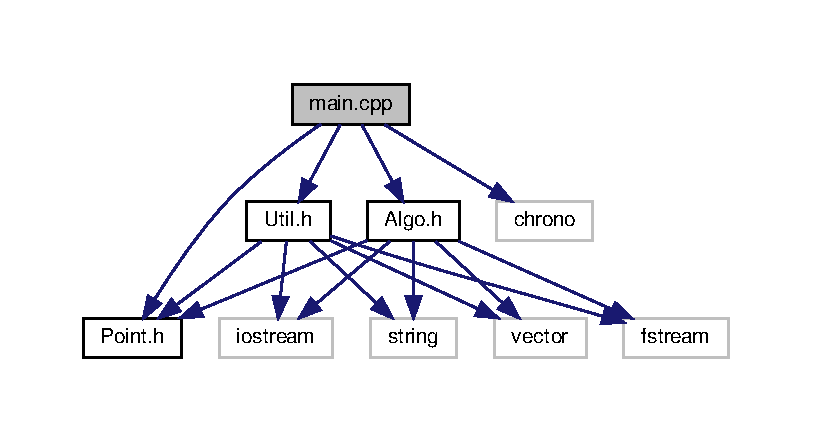
\includegraphics[width=350pt]{main_8cpp__incl}
\end{center}
\end{figure}
\subsection*{Functions}
\begin{DoxyCompactItemize}
\item 
\mbox{\Hypertarget{main_8cpp_a840291bc02cba5474a4cb46a9b9566fe}\label{main_8cpp_a840291bc02cba5474a4cb46a9b9566fe}} 
int {\bfseries main} (void)
\end{DoxyCompactItemize}
\subsection*{Variables}
\begin{DoxyCompactItemize}
\item 
\mbox{\Hypertarget{main_8cpp_a3292ccd664b5d9ece18b54505789e303}\label{main_8cpp_a3292ccd664b5d9ece18b54505789e303}} 
\hyperlink{classAlgo}{Algo} {\bfseries a}
\item 
\mbox{\Hypertarget{main_8cpp_a8f5a671aa7c0bf36152777d06818d290}\label{main_8cpp_a8f5a671aa7c0bf36152777d06818d290}} 
\hyperlink{classUtil}{Util} {\bfseries f}
\end{DoxyCompactItemize}


\subsection{Detailed Description}
This is the base file from which the algorithm is called. 

\begin{DoxyAuthor}{Author}
your name (\href{mailto:you@domain.com}{\tt you@domain.\+com}) 
\end{DoxyAuthor}
\begin{DoxyVersion}{Version}
0.\+1 
\end{DoxyVersion}
\begin{DoxyDate}{Date}
2019-\/03-\/31
\end{DoxyDate}
\begin{DoxyCopyright}{Copyright}
Copyright (cost) 2019 
\end{DoxyCopyright}

\hypertarget{Point_8cpp}{}\section{Point.\+cpp File Reference}
\label{Point_8cpp}\index{Point.\+cpp@{Point.\+cpp}}


\hyperlink{classPoint}{Point} Class.  


{\ttfamily \#include $<$iostream$>$}\newline
{\ttfamily \#include \char`\"{}Point.\+h\char`\"{}}\newline
Include dependency graph for Point.\+cpp\+:
\nopagebreak
\begin{figure}[H]
\begin{center}
\leavevmode
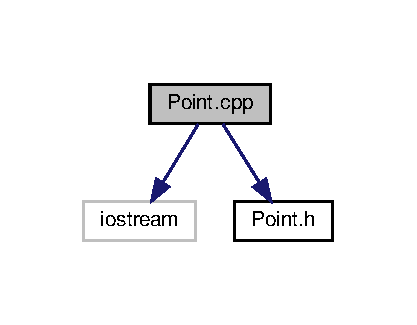
\includegraphics[width=200pt]{Point_8cpp__incl}
\end{center}
\end{figure}


\subsection{Detailed Description}
\hyperlink{classPoint}{Point} Class. 

\begin{DoxyAuthor}{Author}
your name (\href{mailto:you@domain.com}{\tt you@domain.\+com}) 
\end{DoxyAuthor}
\begin{DoxyVersion}{Version}
0.\+1 
\end{DoxyVersion}
\begin{DoxyDate}{Date}
2019-\/03-\/31
\end{DoxyDate}
\begin{DoxyCopyright}{Copyright}
Copyright (cost) 2019 
\end{DoxyCopyright}

\hypertarget{Util_8cpp}{}\section{Util.\+cpp File Reference}
\label{Util_8cpp}\index{Util.\+cpp@{Util.\+cpp}}


\hyperlink{classUtil}{Util} Class which contains the implementation for the segmented least squares algorithm.  


{\ttfamily \#include \char`\"{}Util.\+h\char`\"{}}\newline
{\ttfamily \#include $<$math.\+h$>$}\newline
{\ttfamily \#include $<$algorithm$>$}\newline
{\ttfamily \#include $<$vector$>$}\newline
Include dependency graph for Util.\+cpp\+:
\nopagebreak
\begin{figure}[H]
\begin{center}
\leavevmode
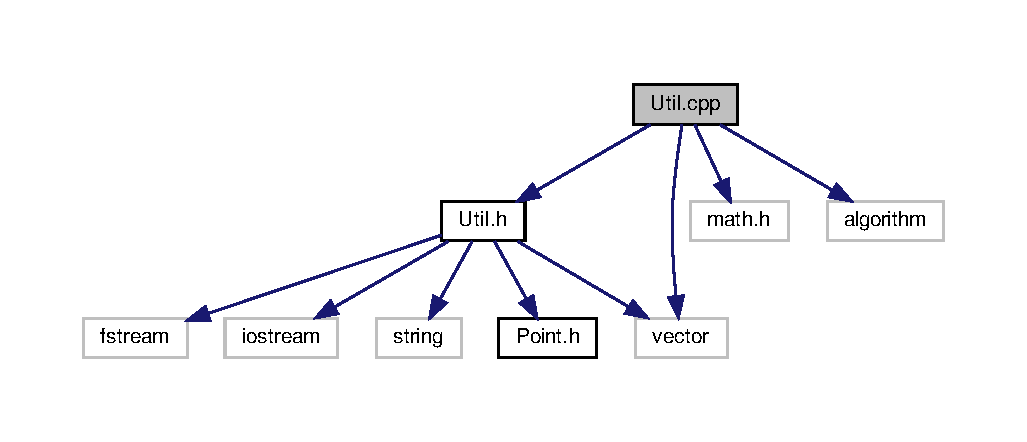
\includegraphics[width=350pt]{Util_8cpp__incl}
\end{center}
\end{figure}
\subsection*{Macros}
\begin{DoxyCompactItemize}
\item 
\mbox{\Hypertarget{Util_8cpp_a12c2040f25d8e3a7b9e1c2024c618cb6}\label{Util_8cpp_a12c2040f25d8e3a7b9e1c2024c618cb6}} 
\#define {\bfseries I\+NF}~numeric\+\_\+limits$<$double$>$\+::infinity()
\end{DoxyCompactItemize}
\subsection*{Functions}
\begin{DoxyCompactItemize}
\item 
bool \hyperlink{Util_8cpp_a12eda38a151ca94e4b50b21d0d6ae028}{comparator} (\hyperlink{classPoint}{Point} p1, \hyperlink{classPoint}{Point} p2)
\begin{DoxyCompactList}\small\item\em Comparator function that compares points by their X co-\/ordinate. \end{DoxyCompactList}\end{DoxyCompactItemize}


\subsection{Detailed Description}
\hyperlink{classUtil}{Util} Class which contains the implementation for the segmented least squares algorithm. 

\hyperlink{classUtil}{Util} Class which contains all the helper functions used in the convex hull algorithms.

\begin{DoxyAuthor}{Author}
your name (\href{mailto:you@domain.com}{\tt you@domain.\+com}) 
\end{DoxyAuthor}
\begin{DoxyVersion}{Version}
0.\+1 
\end{DoxyVersion}
\begin{DoxyDate}{Date}
2019-\/03-\/31
\end{DoxyDate}
\begin{DoxyCopyright}{Copyright}
Copyright (cost) 2019 
\end{DoxyCopyright}


\subsection{Function Documentation}
\mbox{\Hypertarget{Util_8cpp_a12eda38a151ca94e4b50b21d0d6ae028}\label{Util_8cpp_a12eda38a151ca94e4b50b21d0d6ae028}} 
\index{Util.\+cpp@{Util.\+cpp}!comparator@{comparator}}
\index{comparator@{comparator}!Util.\+cpp@{Util.\+cpp}}
\subsubsection{\texorpdfstring{comparator()}{comparator()}}
{\footnotesize\ttfamily bool comparator (\begin{DoxyParamCaption}\item[{\hyperlink{classPoint}{Point}}]{p1,  }\item[{\hyperlink{classPoint}{Point}}]{p2 }\end{DoxyParamCaption})}



Comparator function that compares points by their X co-\/ordinate. 


\begin{DoxyParams}{Parameters}
{\em p1} & \\
\hline
{\em p2} & \\
\hline
\end{DoxyParams}
\begin{DoxyReturn}{Returns}
true 

false 
\end{DoxyReturn}

\hypertarget{Util_8h}{}\section{Util.\+h File Reference}
\label{Util_8h}\index{Util.\+h@{Util.\+h}}


Header file for \hyperlink{classUtil}{Util} Class.  


{\ttfamily \#include $<$fstream$>$}\newline
{\ttfamily \#include $<$iostream$>$}\newline
{\ttfamily \#include $<$string$>$}\newline
{\ttfamily \#include $<$vector$>$}\newline
{\ttfamily \#include \char`\"{}Point.\+h\char`\"{}}\newline
Include dependency graph for Util.\+h\+:
\nopagebreak
\begin{figure}[H]
\begin{center}
\leavevmode
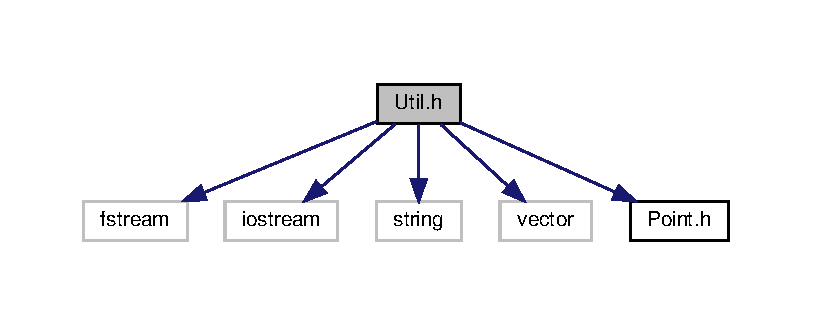
\includegraphics[width=350pt]{Util_8h__incl}
\end{center}
\end{figure}
This graph shows which files directly or indirectly include this file\+:
\nopagebreak
\begin{figure}[H]
\begin{center}
\leavevmode
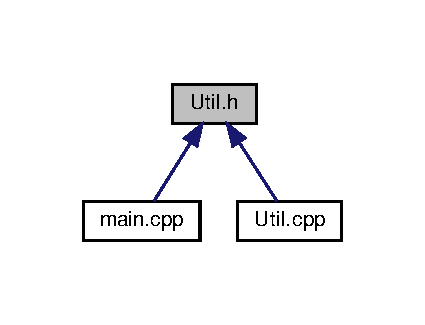
\includegraphics[width=204pt]{Util_8h__dep__incl}
\end{center}
\end{figure}
\subsection*{Classes}
\begin{DoxyCompactItemize}
\item 
class \hyperlink{classUtil}{Util}
\end{DoxyCompactItemize}


\subsection{Detailed Description}
Header file for \hyperlink{classUtil}{Util} Class. 

\begin{DoxyAuthor}{Author}
your name (\href{mailto:you@domain.com}{\tt you@domain.\+com}) 
\end{DoxyAuthor}
\begin{DoxyVersion}{Version}
0.\+1 
\end{DoxyVersion}
\begin{DoxyDate}{Date}
2019-\/03-\/31
\end{DoxyDate}
\begin{DoxyCopyright}{Copyright}
Copyright (cost) 2019 
\end{DoxyCopyright}

%--- End generated contents ---

% Index
\backmatter
\newpage
\phantomsection
\clearemptydoublepage
\addcontentsline{toc}{chapter}{Index}
\printindex

\end{document}
